\chapter{A vezérlést futtató felhő infrastruktúra}
\label{cha:kubernetes}

Ebben a fejezetben rátérünk a felhőrendszer tényleges megvalósítására. A \ref{cha:cloud}. fejezetben megnéztük milyen lehetséges mai technológiák közül választhatunk, realizálhattuk, hogy a Kubernetes tűnik a legjobb választásnak ilyen célra, most pedig ezen a vonalon haladunk tovább. Megnézzük Kubernetesen belül milyen lehetőségek vannak, mik a probléma alapfeltételei és hogyan lehet integrálni a \ref{cha:fizikai}. fejezetben bemutatott konténerkollaborációt egy ilyen Kubernetes felhőbe.

\section{Kubernetes technológiái}
Több Kubernetes technológia közül választhatunk, bepillantunk némelyikbe, hogy mire jó és miért ezt választjuk vagy nem választjuk.

\subsection{K8S}

A K8s a Kubernetes rövidítése ("K", majd 8 "ubernete", majd "s" betű). Azonban általában, amikor az emberek Kubernetesről vagy K8-ról beszélnek, akkor az eredeti upstream projektről beszélnek, amelyet a Google valóban rendkívül elérhető és skálázható platformként tervezett.

Tehát a Kubernetes minden alapfunkcióval, mely összességének tulajdonságai:
\begin{itemize}
	\item elválasztott Master és Worker node-ok, biztosítható az irányítás erőforrása
	\item etcd külön clusteren futtatható, biztosítható a terhelés kezelése
	\item ideális esetben külön bejáratú csomópontokkal rendelkezik, hogy azok könnyedén kezeljék a bejövő forgalmat, még akkor is, ha az alatta lévő csomópontok némelyike foglalt. \cite{k8svsk3s}
\end{itemize}
\subsection{K3S}
A K3S egy egyszerűsített változata a K8S-nek, melynek forrása 40MB bináris fájl, amely teljesen implementálja a Kubernetes API-t. Rengeteg extra driver-t kihagytak belőle, melyre alap esetben nincs szükség tesztrendszer vagy egyszerű klaszter esetén. Ezeket a kihagyott funkciókat egyébként később hozzá lehet illeszteni a rendszerhez add-onokkal. \cite{k8svsk3s}
\subsection{Kind}

A Kind egy Docker fölötti Kubernetes megvalósítás egy node-on. Egyszerű installálni, azonban nem a Kubernetes API-t használja.

\subsection{MiniKube}

A MiniKube az első Kubernetes technológia amely a fejlesztők ajánlása alapján a kezdőknek kipróbálásra a legalkalmasabb. Mivel egyszerű telepíteni, nincs nagy erőforrásigénye (2 vCPU/2GB RAM/20GB lemez). Egy gépre installálható, nem adható több node a klaszterhez. \cite{typesofkubernetes2}

\subsection{Miért K3S?}

A tanszéki klaszter természetesen egy teljes kialakított K8S, melyen az eredeti API használható és teljesértékű szolgáltatásokat lehet tesztelni a Kubernetes összes optimalizálásával. A Kind más API-t használ, így a telepítést leegyszerűsíteni, azonban nem összeegyeztethető egy Kind-os applikáció K8S megvalósításával. MiniKube már egyel jobb, azonban csak egy node-ot használ, ebben a projekben pedig fontos a hálózati tesztelés több node között. Így marad a K3S, amellyel a legjobban szimulálhatjuk a tanszéki K8S rendszert és a megvalósított applikáció is könnyen portolható.

\section{Földi scenario felkészítése a menedzselt felhőrendszerbe}

A felhasznált Docker konténereket néhány esetben változtatni kellett, ez csak a \emph{Dockerfile}-ra igaz, a forráskódok az eredeti esetben is működtek nem K3S rendszeren. Mindegyik konténerben volt egy kivétel, amely csak akkor engedte futtathatóvá tenni a konténert, ha az Docker rendszerben fut, ezt a \emph{[.dockerenv} fájl létezésére vonatkozó feltétel. \\

\noindent
A PX4 szimuláció futtatószkripje (\emph{vke\_px4sim/docker-entrypoint.sh}) ugyan tartalmazza a beépített \emph{ROS\_IP} hirdetőcímet, amelyet a hálózati fejlesztés során többször átírtam, sikerült olyan végeredményre jutni, amelyben az eredeti konténer külső interfész IP-je maradhat. \\

\noindent
Az előkészített Roscore konténert a végleges verzióban nem használom, hiszen egyszerűbb volt az eredeti \emph{alpineros/alpine-ros:noetic-ros-core} publikus image-t megadni, amit a K8S API-ban tudtam testreszabni indított portszámmal és környezeti változókkal.

\section{Kubernetes virtualiztált telepítése}

Egy több node-os klasztert valósítok meg virtualizáció fölött. Virtuális gépek létrehozására rengeteg program létezik, én a Multipass-t választottam. A Multipass egy letisztult VM menedzser Linux-ra, Windows-ra és MacOS-re, amellyel egy parancs indítani és törölni különálló VM-eket bármely CloudInit-et tartalmazó image-ről. Azért választottam ezt, mert könnyedén szkriptelhető a Klaszter törlése és felhúzása, mivel a fejlesztés során sokszor szeretném az alapbeállításról indítani a klasztert. \\

\noindent
Tehát írtam egy Bash scriptet, aminek segítségével létrehozok három VM-et és inicializálom rajtuk a K3S klasztert. Multipass VM-ek létrehozása Bash-ben egy-egy parancs (\ref{lst:mlaunch}. számú kódrészlet), melyek paramétereit természetesen egy config fájlból olvasok be, amiről még később szó lesz.
\begin{minipage}{\linewidth}
\begin{lstlisting}[caption={Multipass VM-ek létrehozása},label={lst:mlaunch}]
multipass launch --name master --cpus 2 --mem 2G --disk 2G
for w in "worker-1 worker-2"; do
	multipass launch --name $slave --cpus 2 --mem 2G --disk 30G
done
\end{lstlisting} 
\end{minipage}
\noindent
Létrehozás után a szkript kiadatja az Apt csomagkezelő program \emph{update és upgrade} parancsait, hogy a legfrissebb Ubuntu 20.04 kompatibilis csomagok legyenek a VM-eken. \\

\noindent
Frissítés után a master VM-en inicializálható a K3S master módban. A parancs eleje azt mutatja, hogy a master nevű VM-en hajtjük végre a "--" utáni parancsokat (\ref{lst:minit}. kódrészlet).
\begin{minipage}{\linewidth}
\begin{lstlisting}[caption={K3S Master inicializálása},label={lst:minit}]
multipass exec master -- /bin/bash -c "curl -sfL https://get.k3s.io | K3S_KUBECONFIG_MODE="644" sh -"
\end{lstlisting}
\end{minipage}
\noindent
Ha ez sikeres, akkor a worker node-okat is inicializálhatjuk, amihez két dologra lesz szükség, a master külső IP-jére, amin keresztül a másik VM tudja elérni, illetve a K3S egyedi tokenre. A master külső IP-jét a multipass egyik parancsából olvassuk ki, a grep programmal rákeresve a master névre, majd az IP cím formátumára reguláris kifejezéssel. A tokenhez szimplán kiíratunk egy fájlt a cat programmal. Ezekkel pedig a master-hez hasonló módon a K3S dokumentációban megadott curl programhívással inicializáljuk a slave-eket. (\ref{lst:initk3s}. kódrészlet)
\begin{minipage}{\linewidth}
\begin{lstlisting}[caption={K3S Slave-ek inicializálása},label={lst:initk3s}]
K3S_TOKEN=$(multipass exec $master sudo cat /var/lib/rancher/k3s/server/node-token)
MASTER_IP=$(multipass list | grep $master | grep -oE "\b([0-9]{1,3}\.){3}[0-9]{1,3}\b")

for slave in $slaves; do
	multipass exec $slave -- /bin/bash -c "curl -sfL https://get.k3s.io | K3S_TOKEN=${K3S_TOKEN} K3S_URL=https://${MASTER_IP}:6443 sh -"
done
\end{lstlisting}
\end{minipage}

\noindent
Sikerességet ellenőrizve a szkiptben még kiíratom a master-en a csatlakozott node-okat.
\begin{lstlisting}[caption={Node-ok lekérdezése}]
multipass exec $master kubectl get nodes
\end{lstlisting}

\section{Konténer képfájlok tárolása}
Docker-Compose esetén a konténer kollaborációs megvalósításhoz elég volt definiálni a könyvtárt, mely forrása és konfigurációja alapján meg kell építeni az image-et és a lokális Docker környezet eltárolta ezen image-eket, amit fel is tudott használni az adott környezetben. Ez természetesnek tűnt, azonban a Kubernetes alapvetően nem tartalmaz ilyen fejlesztéseket, csakis lefordított képfájlokat tud publikus vagy privát registry-ből letölteni. A Docker Registry egy olyan verziókezelő, amely felépített konténer képfájlokat tárol és állít rendelkezésre aktívan használó rendszereknek, mint például a Kubernetes vagy Docker Swarm. Három megoldást próbáltam ki, hogy az egyedi lemezképeket használhassam a felhőmben (\ref{fig:registry}. ábra).\\

\noindent
\paragraph{A)}
Elsőnek úgy gondoltam, hogy a legegyszerűbb megoldás az ha a K3S vagy egy Docker környezetben, amely a K3S master-én futna, inicializálok egy előre készített Docker registry szervert, arra feltöltöm a felépített konténerlemezeket és lokálisan eléri a Kubernetes master, deploy esetén. Tehát definiáltam egy pod-ot, amely az 5000-res porton elérhető a K3S rendszeren belül, a master-ről. A \emph{registry} nevű image-et adtam meg, így a hivatalos Docker registry került letöltésre. Push-olni sikerült konténert, azonban a Kubernetes API-ra definiált Deployment-el már nem sikerült pull-olni SSL biztonsági okok miatt. \\

\noindent
\paragraph{B)}
Ezután hagytam a felhőbe integrálást, a master node-ra telepítettem Dockert és Docker-Compose-t, majd a deploy-oltam a hivatalos oldalról a registry-t (\ref{lst:registryB}. kódrészlet). A konténerek push-olása pedig szintén a master node-ról történt (\ref{lst:localreg} kódrészlet). Ez a megoldás működött, azonban nem túl szép és optimális, mivel a master-en sokszor tárolódik egy konténer image (forrásként, Docker image-ként, Docker registry-ben, Kubernetes letöltött image-ként és példányosított konténerként).
\begin{minipage}{\linewidth}
\begin{lstlisting}[caption={Docker registry inicializálás a master docker környezetében},label={lst:registryB}]
multipass exec ${master} -- sudo docker run -d -p 5000:5000 --restart=always --name registry registry:2
\end{lstlisting}
\end{minipage}
\begin{minipage}{\linewidth}
\begin{lstlisting}[caption={Build és push lokál konténer registry-be},label={lst:localreg}]
for container in "commander px4sim aruco"; do
	multipass exec ${master} -- sudo docker build ${drone_control_dir}/vke_${container}/. -t localhost:5000/${container}
	multipass exec ${master} -- sudo docker push localhost:5000/${container}
done
\end{lstlisting}
\end{minipage}

\paragraph{C)}
Így inkább talán a legegyszerűbb megoldást választottam, igénybe vettem a hivatalos Docker Hub privát repository szolgáltatását, amely ugyan egy konténert biztosít ingyen, egy kis trükkel, mi szerint ugyanazt a konténert töltöm fel 3 különböző taggel, ezt is meg lehet oldani (\ref{lst:registryC}. kódrészlet).
\begin{minipage}{\linewidth}
\begin{lstlisting}[caption={Docker Hub build és push},label={lst:registryC}]
for container in "commander px4sim aruco"; do
	docker build ${drone_control_dir}/vke_${container}/. -t nanasidnl/drone_control:${container}
	docker push nanasidnl/drone_control:${container}
done
\end{lstlisting}
\end{minipage}

 \begin{figure}
 	\centering
 	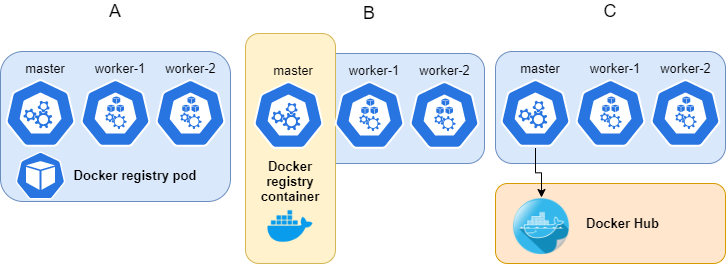
\includegraphics[width=\linewidth]{figures/registry.png}
 	\caption{Registry megoldásaim egyedi konténerek esetén}
 	\label{fig:registry}
 \end{figure}

\noindent
A Docker Hub privát repository-hoz authentikálni kell az API-t, ahhoz hogy elérje az adott K8S deployment. Ehhez egy configurációs fájlba kiszerveztem a hitelesítő adatokat. A szolgáltatást létrehozó deploy szkriptbe pedig beleírtam, hogy használja fel ezt a fájlt és authentikáljon egy \emph{regcred} titkon keresztül (\ref{lst:dhk3s}. kódrészlet). Ezt meg kell adni az API használatakor is (\ref{lst:dhsec}. kódrészlet).
\begin{minipage}{\linewidth}
\begin{lstlisting}[caption={Docker Hub authentikáció K3S-ről},label={lst:dhk3s}]
source ../config/docker-credentials.sh
multipass exec ${master} -- kubectl create secret docker-registry regcred --docker-server=${docker_server} --docker-username=${docker_username} --docker-password=${docker_password} --docker-email=${docker_email}
\end{lstlisting}
\end{minipage}

\begin{minipage}{\linewidth}
\begin{lstlisting}[caption={K8S API secret definiálása a konténerekhez},label={lst:dhsec}]
imagePullSecrets:
- name: regcred
\end{lstlisting}
\end{minipage}


\chapter{Drónirányítás mint szolgáltatás a Kubernetes felhőben}

Az előző (\ref{cha:kubernetes}.) fejezetben megmutattam, hogyan alakítottam ki a saját felhőrendszeremet. Ebben a fejezetben pedig megnézzük a diplomamunkának szánt feladat miként tud felkerülni ebbe a felhőbe. Végignézzük a Kubernetes API szolgáltatásait, mely technológiával mit lehet elérni a cél érdekében. Kezdjük a legegyszerűbb Pod-tól és betekintünk az API szolgáltatásainak jelentős részébe.

\section{Szimpla 4 podos megvalósítás}
Elsőként a legegyszerűbb összeállításban szerettem volna megbizonyosodni arról, hogy a szolgáltatás valóban tud működni a felhőben ezért elsőnek a négy konténert 4 különálló pod-ként próbáltam ki (\ref{lst:1pod4}. kódrészlet). \\

\noindent
A Pod a legkisebb telepíthető számítási egység, amely létrehozható és kezelhető a Kubernetesben. Egy Pod létrehozása esetén példányosodik az előre definiált konténer vagy konténer csoport, azonban a futás megkezdése után semmilyen felügyeleti szolgáltatásban nem részesül, nem indul újra leállás esetén, nem alkalmazódik rá semmilyen skálázás. Egyszerűen ha csak Pod szinten futtatunk alkalmazásokat, akkor ugyanott járunk mintha Docker Swarm környezetben dolgoznánk. \\
\begin{minipage}{\linewidth}
\begin{lstlisting}[caption={Példa egy Pod-ra a négyből},label={lst:1pod4}]
apiVersion: v1
kind: Pod
metadata:
	name: aruco
	labels:
		name: drone-hq
spec:
	hostname: aruco
	containers:
	- 	image: nanasidnl/drone_control:aruco
		name: aruco
	env:
	- 	name: ROS_MASTER_URI
		value: "http://roscore:11311"
	- 	name: ARUCO_LAUNCH
		value: "sim"
	imagePullSecrets:
	-	name: regcred
\end{lstlisting}
\end{minipage}

\noindent
Jelen négy Podos megvalósításban a belső hálózati problémák nem merültek fel, hiszen a Pod neve hostname-ként is funkcionál, így egymás között könnyedén el tudták érni egymást az alkalmazások. Ez egy működő verzió volt, azonban túl egyszerű. A drón szimulációt nem a felhőben képzeljük el, hiszen a fizikai drón sem a felhőben fog futni.

\section{Konténerek hálózata, Service és Deployment}

Ahhoz, hogy a Kubernetes szolgáltatásait érdemben igénybe tudjuk venni valamilyen magasabb szintű API-t kell használnunk. Ezért megnézzük a Deploymentet és a Service-t. Utóbbi arra szolgál, hogy a szolgáltatásunk megfelelő külső interface-el rendelkezhessen, bármely mögöttes konténerkonstrukcióval, amely integritását a Deployment biztosítja. Mindegyik Pod megkapja a saját IP-címét, azonban egy Deployment során az egy pillanatban futó Podok halmaza eltérhet az adott alkalmazást egy időpillanattal később futtató Podok halmazától. A nem natív alkalmazások esetében a Kubernetes lehetőséget kínál hálózati port vagy LoadBalancer elhelyezésére az alkalmazás és a háttéralkalmazások között. \cite{kservice} \\

\begin{minipage}{\linewidth}
\begin{lstlisting}[caption={Példa 4 konténeres deployment megoldásra},label={lst:4deploy}]
apiVersion: apps/v1
kind: Deployment
metadata:
	name: drone-hq
spec:
	replicas: 1
	selector:
		matchLabels:
			app: drone-hq
	template:
		metadata:
			labels:
				app: drone-hq
	spec:
	containers:
	-	name: roscore
		image: alpineros/alpine-ros:noetic-ros-core 
	-	name: aruco
		image: nanasidnl/drone_control:aruco
	- 	name: commander
		image: nanasidnl/drone_control:commander
			ports: 
			-	containerPort: 80
		image: nanasidnl/drone_control:px4sim
			ports: 
			- containerPort: 10000
	imagePullSecrets:
	-	name: regcred
\end{lstlisting}
\end{minipage}

\noindent
Elsőnek a 4 podos verzióból készítettem egy Deploymentet (\ref{lst:4deploy}. kódrészlet), amely már egy Pod-ként definiálható, azonban érvényesülni fognak rá a Kubernetes integritás szabályai. A Roscore konténert éri el az összes, de Pod-on belüli kommunikáció a legkönnyebb, hiszen egy Pod egy lokális hálózatnak szármoztatható le, így a konténerek \emph{localhost}-ra címezve tudnak kommunikálni egymással, mintha virtuális környezetben lennének. Külső interfész 2 van, a Gazebo szimuláció és az irányító dashboard. \\

\begin{minipage}{\linewidth}
\begin{lstlisting}[caption={Példa 4 konténeres megoldás service kivezetésére},label={lst:4service}]
apiVersion: apps/v1
kind: Service
metadata:
	name: drone-hq
spec:
	ports:
	-	port: 80
		targetPort: 81
		name: dashboard
	-	port: 10000
		targetPort: 10001
		name: gazebo
\end{lstlisting}
\end{minipage}

\noindent
A külső interface-ek kapcsán jön képbe a Service API, míg minden belső kommunikációt le tud kezelni a Deployment, ahhoz hogy ezeket a külső interface-eket elérjük kell definiálnunk egy Service-t a Deployment fölé (\ref{lst:4service}. kódrészlet), amely a Deployment selectorán keresztül kapcsolódik hozzá és a definiált portokhoz rendel egy külső portot. Ez a külső port valjában csak a Kubernetes rendszeren definiált flannel hálózatról elérhető. Tehát más a rendszeren futó alkalmazás el fogja tudni érni, de kívülről nem. Márpedig a fizikai drón irányításra tervezünk, így következő lépésként a befelé való kommunikáció megvalósíthatósági technológiáit fogjuk megvizsgálni.

\section{Szolgáltatás külső elérése}
Több Kubernetes API szolgáltatás rendelkezésünkre áll, hogy elérhessük kívülről a konténerünket amin a felhasználói felület fut, illetve a drónnak kivezessük a roscore konténer Mavlink protját.

\subsection{NodePort}
A NodePort szolgáltatás a legprimitívebb módja a külső forgalom közvetlenül a szolgáltatásának elérésére. A NodePort, amint a neve is mutatja, megnyit egy adott portot az összes csomóponton (a virtuális gépek), és az erre a portra küldött forgalmat továbbítja a szolgáltatásnak. \cite{nodeport} A NodePortokat hasonlóan rendelhetjük hozzá a szolgáltatás portjaihoz, mint a sima proxy-n keresztüli külső portot, azonban a NodePort számozása 30000-től kezdődhet. \\

\noindent
Ezzel a megoldással meghatározhatjuk, hogy a drón kívülről a Master külső IP-jén érjen el minden szükséges alkalmazást, illetve a drónt irányító személy is érje el a Dashboard-ot. A probléma a NodePort-tal, hogy más porton nem tud kommunikálni, így a Roscore véletlenszerűen generált portja nem lesz elérhető kívülről.

\begin{minipage}{\linewidth}
\begin{lstlisting}[caption={Service kiegészítése NodePort-okkal},label={lst:nodeport}]
apiVersion: v1
kind: Service
metadata:
	name: drone-hq
spec:
	type: NodePort
	ports:
	-	port: 80
		nodePort: 30080
		name: dashboard
	-	port: 11311
		nodePort: 31311
		name: roscore
selector:
	app: drone-hq
\end{lstlisting}
\end{minipage}

\subsection{Ingress, szolgálgatások szétválasztása}
Fontos megemlíteni az Ingress-t is, hiszen több alkalmazásban gondolkozunk, mivel lesz két konténerünk a felhőben amelyből egy példányt szeretnénk és a Roscore-t egészíti ki, ezt neveztem \emph{drone-hq}-nak, ez tartalmazza az aruco kódolvasót és az irányítót. A másik pedig a Roscore, amiből szeretnénk backup futó szolgáltatást. Ha hosszútávú szolgáltatást szeretnénk alakítani vagy továbbfejleszteni, esetleg publikus felhőben, akkor mindenképpen érdemes az Ingress-t használni, mivel domain-eket, subdomain-eket és útvonalakat rendelhetünk a különböző szolgáltatásunk felé (\ref{fig:ingress}. ábra). Így ha publikus felhőben gondolkoznánk, akkor a roscore backup-okat ki lehetne vezetni különböző elérési címekre, illetve változtathatnánk a címek mögöttes elérését, ha szükséges.

\begin{figure}
	\centering
	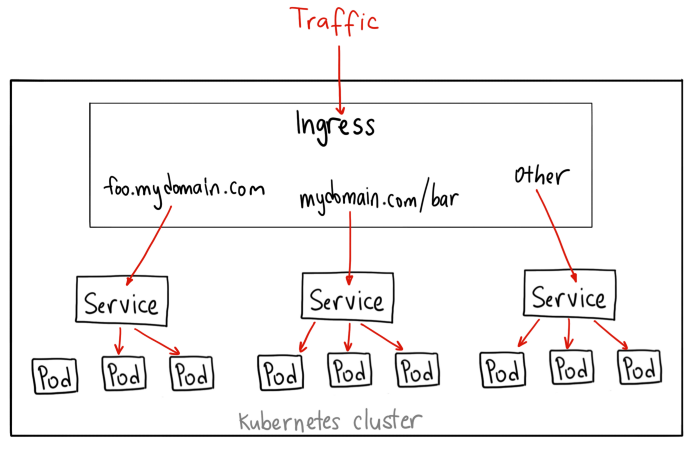
\includegraphics[width=\linewidth]{figures/ingress.png}
	\caption{Ingress Service szétválasztása a klaszterben \cite{nodeport}}
	\label{fig:ingress}
\end{figure}

\subsection{ROS Port forwarding}
Az Ingress megoldás biztosíthatná, hogy szétválasszuk a Roscore-t és a többi konténert a magasabb rendelkezésre állás érdekében, azonban a Roscore rendelkezik egy nem túl előnyös kommunikációs kapcsolódási stratégiával. Egy ROS rendszer működtethet számtalan eszközt, a mi példánkban egy Roscore-ra három ROS Node csatlakozik, egyedül a drón a felhőn kívülről (\ref{fig:rosjoin}. ábra). Mikor elsőnek csatlakozik egy Node, akkor megkap bizonyos paramétereket, mint például a portszám amin az adott node-nak kommunikálnia kell a Roscore-ral. Felmerül a kérdés, hogy a külső ROS Node hogyan fog bejutni a Kubernetes cluster szolgáltatásához véletlenszerűen generált porton. \\

\noindent
Sokféle megoldáson gondolkoztam, azonban mivel egy egyszerű NAT-olt hálózat mögé is csak úgy lehet elhelyezni a kiszolgáló Roscore-t ha az lérhető portok intervallumát kinyitjuk a nagyvilág felé, mivel nem előre tudható, hogy milyen portot fog lefoglalni az adott Node-al való kommunikációra. Ezt részletesen bizonyítja a \cite{portforward} számú hivatkozott cikk. Gondoltam olyan megoldásra is amely korlátozza a Linux alapú konténer által kiosztott portszámot a Roscore alatt. Ezt úgy lehetne megoldani a Roscore konténer inicializálásnál lekorlátozom a kiosztható portokat a NodePort tartományra, ami 30000 és 32767 között van (\ref{lst:portlimit}. kódrészlet). Majd amikor a külső eszköz felveszi a kommunikációt, akkor a logban kap egy hibát "\emph{ERROR: Communication with node[http://10.42.2.13:32045/] failed!}", amelyből ki tudjuk olvasni a portszámot és kinyithatjuk ezt a NodePortot. Ez azért visszás, mert súlyos másodpercek telnek el, amíg megkapjuk a hibaüzenetet, felolvassuk és eljuttatjuk a dróntól a klaszterig. Így ezt a megoldást QoS célú szolgáltatás alatt nem engedhetjük meg.

\begin{lstlisting}[caption={Linuxon kiosztható port korlátozása}, label={lst:portlimit}]
echo 30000-32767 > /proc/sys/net/ipv4/ip_local_reserved_ports
\end{lstlisting}

\begin{figure}
	\centering
	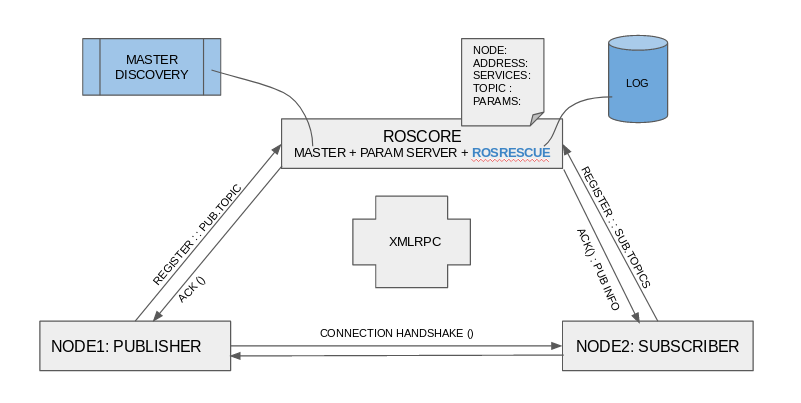
\includegraphics[width=\linewidth]{figures/rosjoin.png}
	\caption{ROS Node csatlakozása Roscore-hoz \cite{rosjoin}}
	\label{fig:rosjoin}
\end{figure}

\subsection{LoadBalancer}
A valódi megoldást a LoadBalancer fogja nyújtani, ami egy standard megoldás arra, hogy egy teljes szolgáltatást kiirányítsunk a klaszterből, a teljes port intervallumon, amelyet a Roscore generálhat. Ez a port az egyik Node-on lesz elérhető, amelyiken az adott Pod fut. A LoadBalancert használhatjuk NodePort-tal is, ami a mögöttes alkalmazásunknak megfelel, hiszen onnan csak egy konstans portra van szükségünk, hogy a felhasználó elérhesse az irányító felületet. Tehát a LoadBalancer segít abban, hogy az elválasztott Roscore szolgáltatás egyedi Node elérésével legyen elérhető, továbbá lehetővéteszi, hogy különböző drónok Roscore-ja ugyanazon a Node-on fussanak és legyenek elérhetőek egymás mellett. A magok elsőkénti elérése inkrementális sorrendben fog történni az alapértelmezett porttól, a további kommunikáció pedig a kisorsolt egyedi portokon (\ref{fig:loadbalancer}. ábra). \\

\begin{minipage}{\linewidth}
\begin{lstlisting}[caption={Roscore Service specifikációja inkrementális változókkal}, label={lst:kubeload}]
spec:
	hostname: roscore-$(DRONE_IDENTIFIER)
	containers:
	-	name: roscore-$(DRONE_IDENTIFIER)
		image: alpineros/alpine-ros:noetic-ros-core 
		env:
		-	name: ROS_IP
			valueFrom:
				fieldRef:
					fieldPath: status.podIP
		-	name: ROS_MASTER_URI
			value: "http://$(ROS_IP):$(MAVLINK_PORT)"
		args: ["roscore", "-p", "$(MAVLINK_PORT)"]
	hostNetwork: true
\end{lstlisting}
\end{minipage}

\noindent
A K8S megvalósításhoz a szolgáltatás yaml fájlt kell módosítanunk az adott Service-hez (\ref{lst:kubeload}. kódrészlet). Automatikusan deployoló szkriptekkel dolgoztam, így a yaml fájlokban megtalálható \emph{\$(VARIABLE)} formátúmú változókat a klaszterhez való hozzáadás előtt adom meg. A \emph{DRONE\_IDENTIFIER} a drón azonosítója, egytől indulunk, ez alapján számoljuk ki a pontos portokat. A \emph{ROS\_IP} a konténer belső változója, amely a ROS Node-ok számára hirdetendő kapcsolattartó IP címet adja meg, a fájlban látható módon kivezettem, hogy a Kubernetes status.podIP változója legyen, tehát a Pod külső IP címe. A \emph{ROS\_MASTER\_URI} pedig az a HTTP cím melyen kapcsolódni tud a ROS Node a core-hoz. A konténert nem hagyományos módon indítjuk, hanem a kiválasztott \emph{MAVLINK\_PORT} hirdető porton, melyet deploy során fog megkapni. \\

\begin{figure}
	\centering
	\includegraphics[width=\linewidth]{figures/loadBalancer.png}
	\caption{LoadBalancer megoldás Kubernetes felhőben}
	\label{fig:loadbalancer}
\end{figure}

\noindent
Ennél a pontnál vettem észre először a K3S hiányosságát, ugyanis a K8S alapból tartalmazza a Traefik modult, amely egy Ingress Controller-rel egybeépített LoadBalancer megvalósítás. A LoadBalancer használatához pedig szükséges hozzáadnunk utólag ezt a modult klaszterhez. Így a K3S-t installáló szkriptet kiegészítettem a Traefik pod-ként való hozzáadásával a klaszterhez (\ref{lst:traefik}. kódrészlet).

\begin{lstlisting}[caption={Traefik hozzáadása a klaszterhez}, label={lst:traefik}]
multipass exec $master -- sudo kubectl apply -f /var/lib/rancher/k3s/server/manifests/traefik.yaml
\end{lstlisting}

\section{Teljes klaszter létrehozása N drónnal}

\subsection{Kauzalitási probléma}
Szimulációnk létrehozásához több különálló lépést kell megtennünk, miután üzemképes a K3S/K8S klaszter. Nézzük meg milyen információ függőségei vannak az egyes komponenseknek.
\begin{itemize}
	\item A drónnak tudnia kell a Roscore-t futtató Node külső IP-jét
	\item Az irányító konténernek ismernie kell a drón IP címét
\end{itemize}

\noindent
Ezen feltételekből következik a kialakított sorrendem, hogy hogyan inicializáljuk a virtuális tesztkörnyezetet. A diplomatervhez csatolt forráskód \emph{deploy} könyvtárában sorszámozással megtalálhatóak ezek Bash szkriptek formájában.

\begin{enumerate}
	\item K3S klaszter létrehozása, kimenet: master és worker-ek IP címei
	\item ROSCore-ok indítása a klaszteren, kimenet: melyik drón-hoz tartozó core melyik Node-ra került
	\item Drónok indítása, külső környezetben (Docker), kimenet: drónok IP címei
	\item Drone-HQ indítása a klaszteren
\end{enumerate}
A lépések végrehajtása után feláll a teljes rendszer és a drónok irányíthatóak a master külső IP-jén keresztül.

\section{Telepítési szkriptek}
Az előző felsorolásból kimaradt egy nulladik szkript, amely arra szolgál, hogy a legfrissebb verziójú konténereket felépíti és feltölti a DockerHub-ra, privát repository-ba. A szkriptek egy közös konfigfájlt használnak \emph{config}), amely-ben a klaszter paraméterei, kezdő portszámok és a drónok száma szerepel. Ezt a konfigfájlt használja Bash és Python program is, ezért a Bash felkonfigurálására létrehoztam egy kiegészítő szkriptet (configUp.sh), amely lemenedzseli a mapparendszerből következő változókat, hogy mi hol van, erre csak a Bash szkripteknek van szüksége. Utána minden deploy szkript ezt a külső konfigurációt hívja meg és konzisztens változókat fognak használni. \\

\noindent
A megoldásom két sablonfájlt tartalmaz a forrás \emph{kubernetes} könyvtárában, \emph{kube-roscore.yml} és \emph{kube-drone-hq.yml}. Mindkét fájl tartalmaz környezeti változókat, melyek értékét az adott drón azonosítószámában találhatunk ki. Ugyan a környezeti változókat tudná kezelni a Kubernetes API, a Multipass rendszeren keresztül viszont ha létrehozzuk az adott Service-t, akkor a master környezeti változóit használná fel, amit a Multipass rendszerén keresztül nem tudunk beállítani. Így ezekből a yaml fájlokból létrehoz a szkript annyit amennyi drón szerepel a konfigurációban. Ezután a Linuxos sed program segítségével cseréljük ki a környezeti változókat Bash változó értékekre. Ahhoz, hogy a gazdagép fájlrendszeréből fel tudja használni a virtuális master a yaml fájlt, a Multipass segítségével mount-olom a könyvtárat a végrehajtás előtt (példa: \ref{lst:script}. kódrészlet). A példában az látszik, hogy a mount parancs után információkat gyűjtünk, a konfigurációból szármozik a Roscore node neve, ami kap egy címkét, majd ez alapján megkeressük a Multipass listázásával a külső IP-jét, hasonlóan a master-nek. Ez után minden drónra elvégezvén (for cikusban), kiszámítjuk az adott drón Mavlink csatlakozási portját, lemásoljuk a sablonfájlt és a már említett környezeti változókat kicseréljük benne, végül a \emph{kubectl apply} paranccsal elindítjuk a klaszteren. \\

\begin{minipage}{\linewidth}
\begin{lstlisting}[caption={Roscore információk összegyűjtése és deploy},label={lst:script}]
multipass mount ${work_dir} ${master}
multipass exec $master -- kubectl label nodes ${ROSCORE_NODE} dedicated=roscore
MASTER_IP=$(multipass list | grep $master | grep -oE "\b([0-9]{1,3}\.){3}[0-9]{1,3}\b")
ROSCORE_IP=$(multipass list | grep $ROSCORE_NODE | grep -oE "\b([0-9]{1,3}\.){3}[0-9]{1,3}\b")
for i in $(seq 1 ${NUMBER_OF_DRONES}); do
	MAVLINK_PORT=$((i-1+MAVLINK_START_PORT))
	cp ${service_dir}/kube-roscore.yml ${service_dir}/kube-roscore-$i.yml
	sed -i 's/$(MAVLINK_PORT)/'${MAVLINK_PORT}'/g' ${service_dir}/kube-roscore-$i.yml
	sed -i 's/$(DRONE_IDENTIFIER)/'${i}'/g' ${service_dir}/kube-roscore-$i.yml
	multipass exec ${master} -- sudo kubectl apply -f ${service_dir}/kube-roscore-$i.yml
done
\end{lstlisting}
\end{minipage}

\noindent
A Roscore deploy szkriptjéhez nagyon hasonló a drónokat indító szkript és a Drone-HQ-t indíti szkript. A drónok indításánál Docker megoldást alkalmazok a külső környezetben, ahol hasonlóan szármoznak le az adott információk, a szimuláció külső portja is hasonlóan inkrementális a Mavlink porthoz (\ref{lst:dronedeploy}. kódrészlet). A Roscore címét a master-en keresztül kapjuk meg, a \emph{kubectl get pods - wide} parancs standard kimenetéből kiolvasva grep programmal, először az elnevezett Service nevére szűrve, utána az IP formátumra. A drón indítása Docker paranccsal történik, ahol megadjuk a környezeti változókat, melyeket alapján el fogja érni az adott Roscore-t, illetve a dashboard-ot átirányítjuk a 10000-res portról inkrementálisan, hogy akármennyi drónt lehessen irányítani.

\begin{minipage}{\linewidth}
\begin{lstlisting}[caption={Drónok indítása külső Docker környezetben}, label={lst:dronedeploy}]
for i in $(seq 1 ${NUMBER_OF_DRONES}); do
	ROSCORE_IP=$(multipass exec $master -- kubectl get pods -o wide | grep roscore-$i | tail -n 1 | grep -oE "\b([0-9]{1,3}\.){3}[0-9]{1,3}\b")
	MAVLINK_PORT=$((i-1+MAVLINK_START_PORT))
	SIMULATION_PORT=$((i-1+SIMULATION_START_PORT))

	docker run --name drone-$i -e ROS_IP=${ROSCORE_IP} -e ROS_MASTER_URI=http://${ROSCORE_IP}:${MAVLINK_PORT} -p ${SIMULATION_PORT}:10000 -d nanasidnl/drone_control:px4sim
done
\end{lstlisting}
\end{minipage}

\noindent
Egy teljesen felépített két drónos rendszer a \ref{fig:full2drone}. ábrán látszik. Az egy fizikai gépes környezetben a három Multipass VM-en a K3S rendszer látható, mellette ugyanabban a környezetben a Docker, amin keresztül a két szimuláció fut. A K3S klaszteren belül a három Node-on öt Pod-ot láthatunk, a Traefik alkalmazást, ami a Roscore LoadBalancer-e miatt szükséges, illetve a két-két drón kiszolgáló Pod-ot. A szimuláció konténerei a Multipass külső IP címein a hozzájuk tartozó porton érik el a Roscore-t. Az irányító lehet az adott környezetben, de akár a hálózaton más fizikai környezetben is, csak el kell érnie az alkalmazásokat az adott portokon.

\begin{figure}
	\centering
	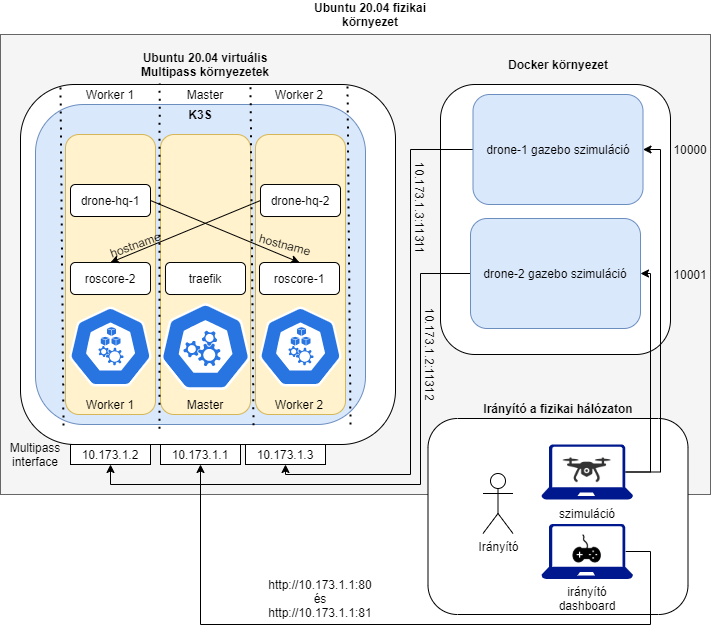
\includegraphics[width=\linewidth]{figures/full2drone.png}
	\caption{Teljes környezet két szimulációval}
	\label{fig:full2drone}
\end{figure}